\chapter{Market Analysis}
\label{sec:market}

In order to evaluate AndroMEDA effectiveness in identifying malware, it's important to evaluate the ability to identify malware without it. As previously discussed in \ref{sec:permissions}, Permissions are the single security measure that defends an Android user from malicious software. We hope to show a fundamental disconnect between Permissions and UAA, as conclusive evidence that Permissions should not be the sole security system on Android. In order to study this, we must examine the how Permissions reflect app behavior, and if known malware can be identified with Permissions alone.



\begin{table*}[t]
\begin{small}
\begin{tabular}{r|l}
Metadata & Description \\
\hline

\textit{App Name} & The name of the app, e.g. Google Maps  \\
\textit{App Developer} & The name of the developer, e.g. Google  \\
\textit{Android Version} & The lowest compatible Android version  \\
\textit{Number of Installs} &  The total number of installs. Given as a range. \\
\textit{Description} &  A long (3000 word max) description of the app. \\
\textit{Reviews} &  The user reviews of the app. \\
\textit{Overall Rating} &  The overall rating of the app, from 1 to 5. A user does not need to write a review to leave a rating. \\
\textit{Requested Permissions} &  The list of all the permissions the app requests. \\

\end{tabular}
\end{small}
%\vspace{-0.2in}
\caption{Metadata from \temp{AndroidMarketDB}}
\label{tab:marketmetadata}
%\vspace{-0.1in}
\end{table*}


\section{Market Dataset}
To do a broad scale study of Android permissions, we introduce a novel dataset: \temp{AndroidMarketDB}. \temp{AndroidMarketDB} contains metadata from \temp{80\%} of all known Android Apps in the GPStore. This metadata, described in \ref{tab:marketmetadata}, is rich in contextual information about an app. For a period of 1 month in May-June 2012, the GPStore was scanned twice a day. This dataset provides detailed metadata for all areas of the Android market, not just the top percent. Despite the large amount of metadata available, we will focus on the Permissions, leaving most other fields for Future Work\ref{sec:futurework}.



\section{Global Permission Analysis}
We first look at the global trends of Permissions in the GPStore. Ideally, all malicious behavior would show up in the permission fingerprint of an app, so therefore it's unique set of capabilties would stand out in the Google Play Store. Ultimately, however, we expect this method to have it's shortcomings.

\begin{figure}[t]
\begin{center}
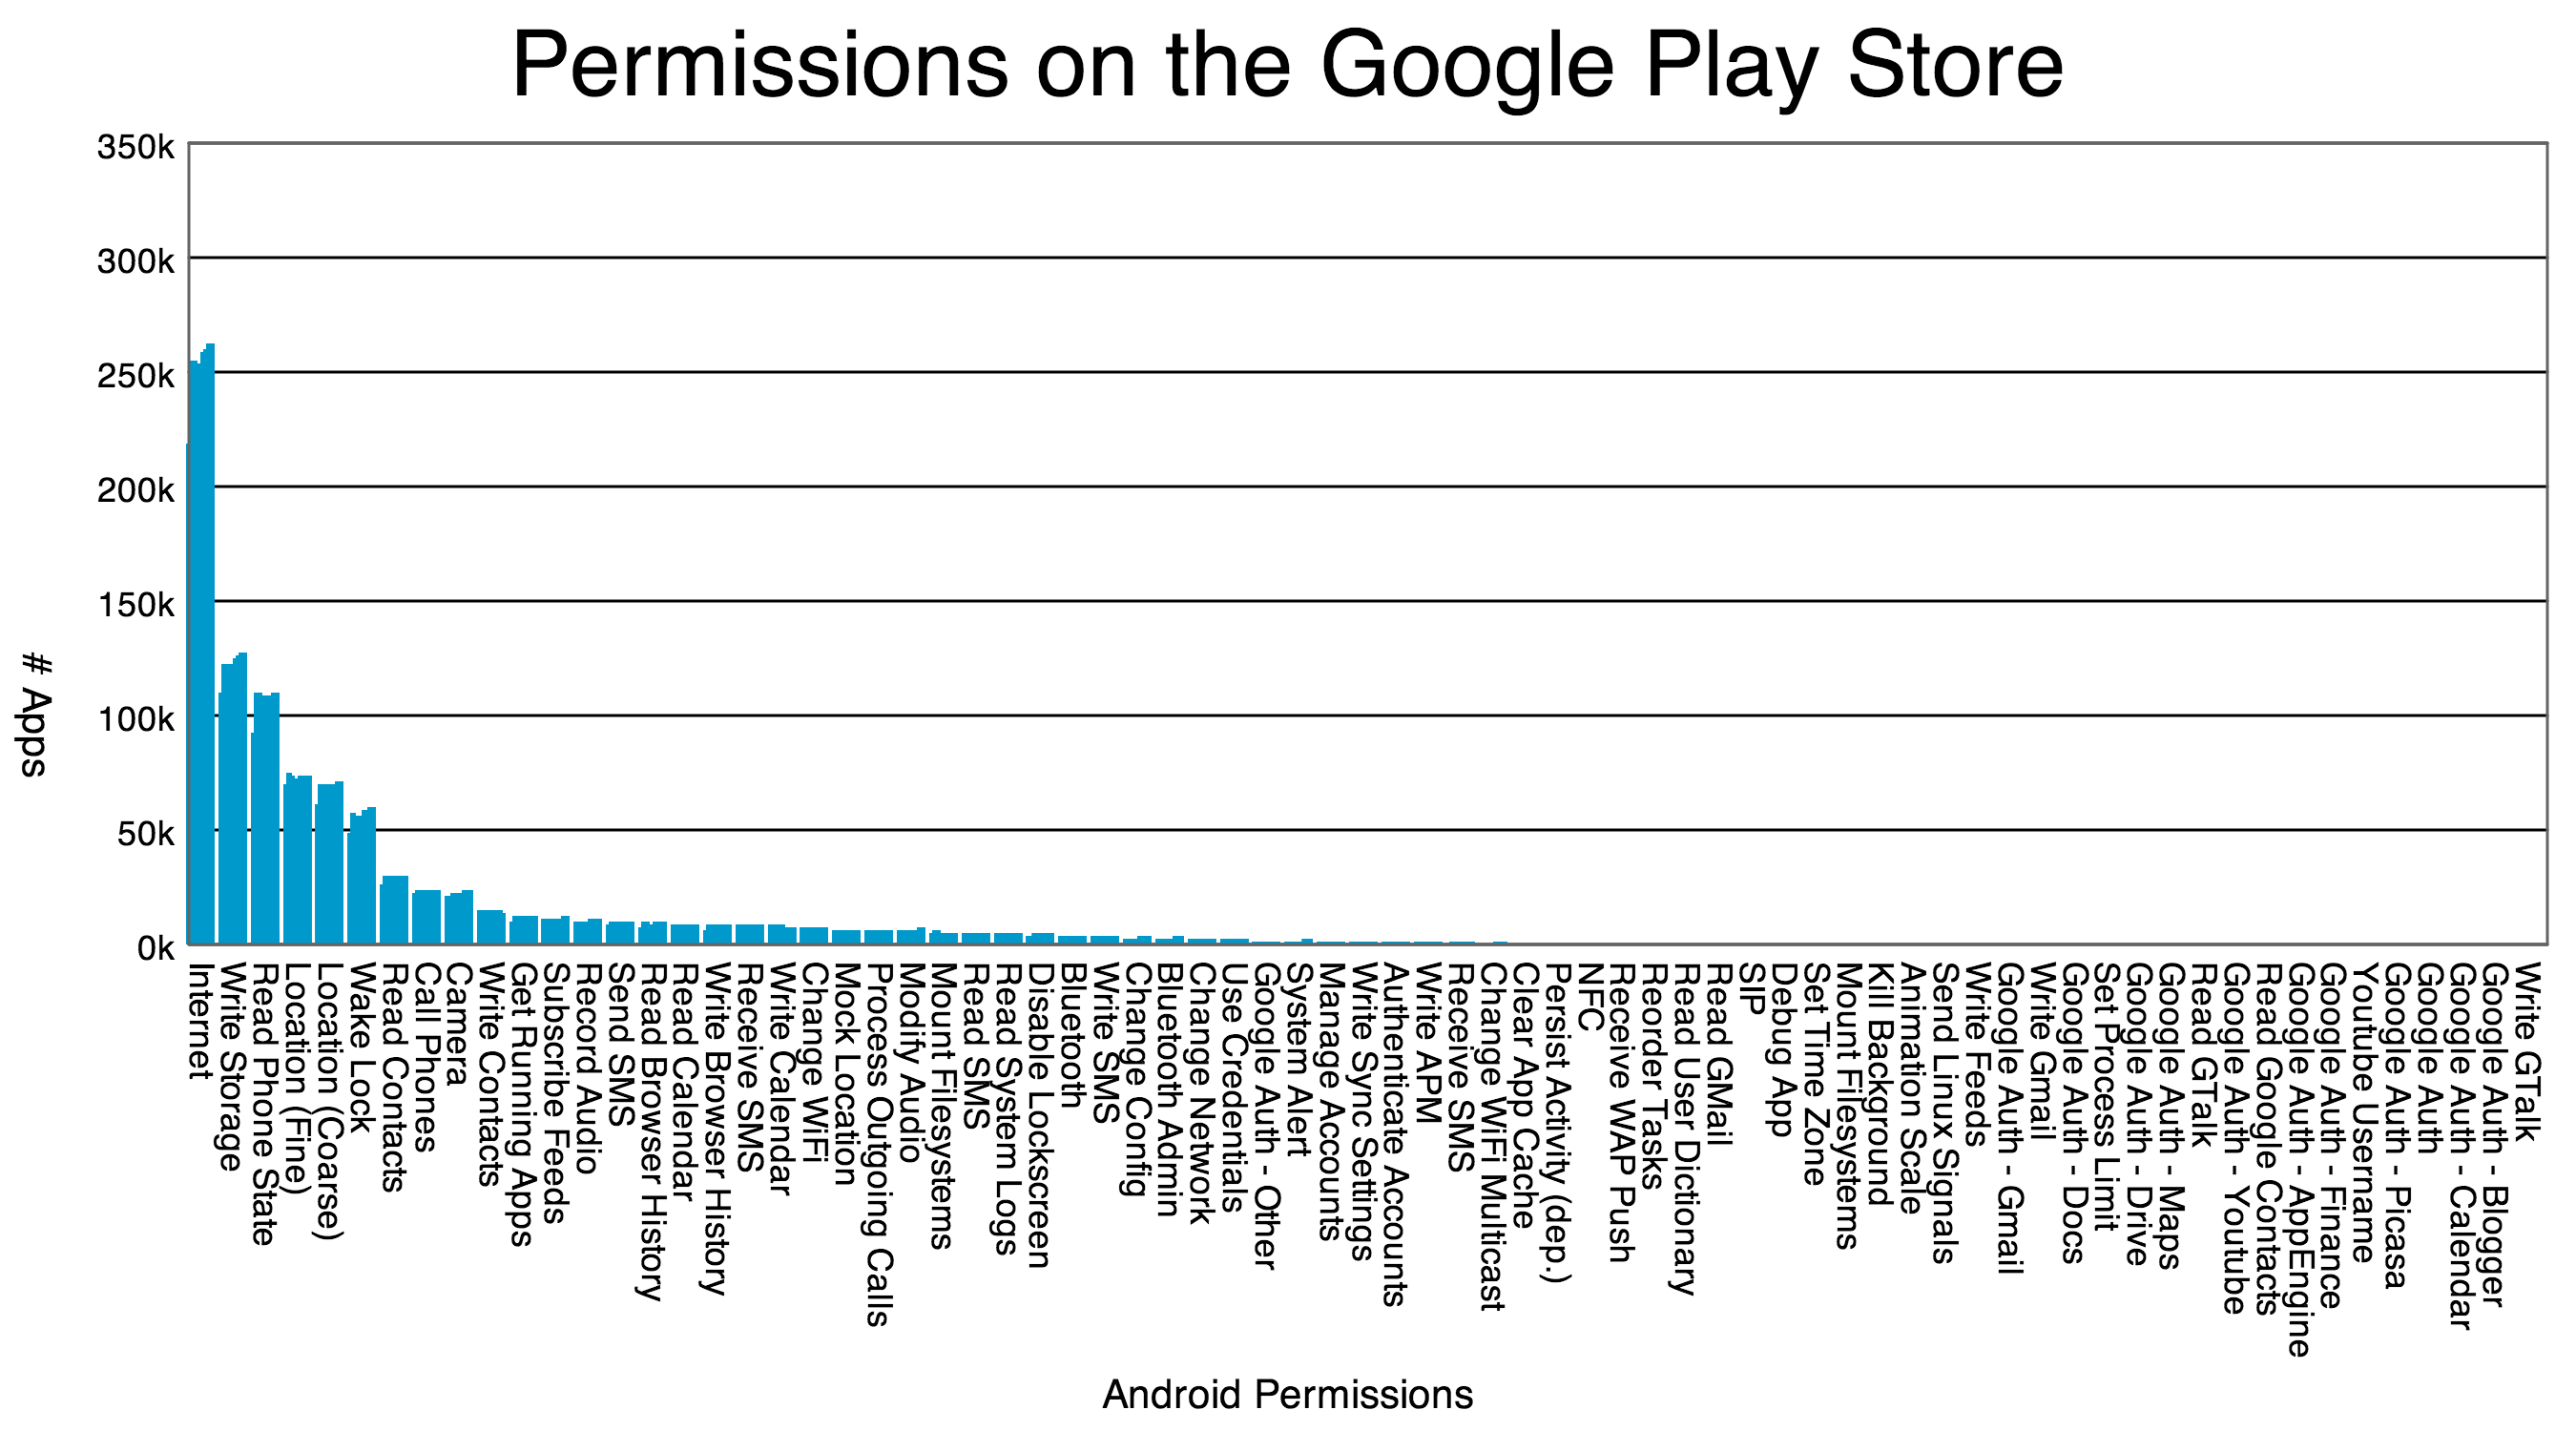
\includegraphics[width=1.0\columnwidth]{figs/AllPermissions}
\caption{Permissions, sorted by how many apps request them in the entire GPStore dataset}
\label{fig:allpermissions}
\end{center}
\end{figure}
